%https://www.uptodate.com/contents/active-surveillance-for-men-with-clinically-localized-prostate-cancer#H4034362282
%https://ascopost.com/issues/july-25-2019/active-surveillance-for-early-stage-prostate-cancer-requires-active-participation-by-patient-and-clinician/

% !TEX root =  ../main_manuscript.tex 
\section{Introduction}
Patients with low- and very low-risk screening-detected localized prostate cancer are recommended active surveillance (AS) usually, instead of immediate radical treatment~\citep{briganti2018active}. In AS, cancer progression is monitored routinely via prostate-specific antigen (PSA), digital rectal examination (DRE), repeat biopsies, and recently, magnetic resonance imaging (MRI). Among these, the strongest indicator of cancer-related outcomes is the biopsy Gleason grade group~\citep{epsteinGG2014}. When it increases from group~1 (Gleason 3+3) to 2 (Gleason 3+4) or higher, it is called \emph{upgrading}~\citep{bruinsma2017expert}. Upgrading is an important endpoint in AS upon which patients are commonly advised curative treatment~\citep{bul2013active}.

Biopsies in AS are always conducted with a time gap between them. Consequently, upgrading is always detected with a time delay (Figure~\ref{fig:delay_explanation}) that cannot be measured directly. In this regard, to detect upgrading timely, many patients are prescribed fixed and frequent biopsies, most often annually~\cite{loeb2014heterogeneity}. However, such one-size-fits-all schedules lead to unnecessary biopsies in slow/non-progressing patients. Biopsies are invasive, may be painful, and are prone to medical complications such as bleeding and septicemia\citep{loeb2013systematic}. Thus, biopsy burden and patient non-compliance to frequent biopsies~\citep{bokhorst2015compliance} have raised concerns regarding the optimal biopsy schedule~\citep{inoue2018comparative, bratt2013study} in AS.

\begin{figure}
\centerline{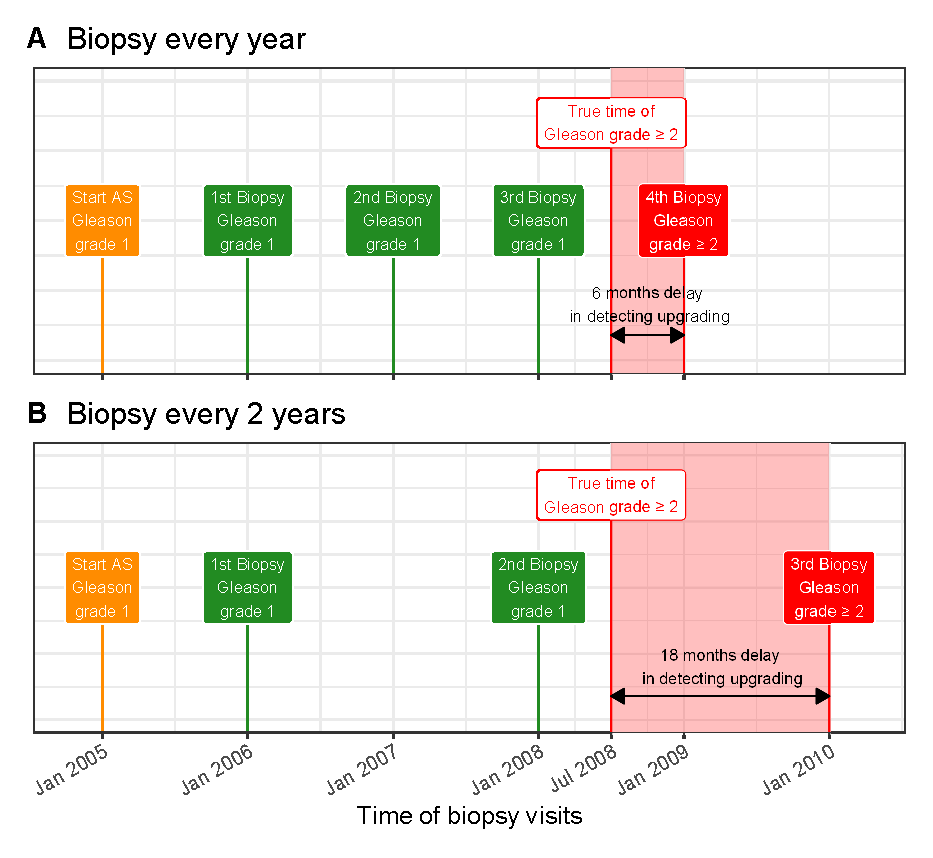
\includegraphics[width=\columnwidth]{images/delay_explanation.eps}}
\caption{\textbf{Trade-off between the timing and number of biopsies (burden) and time delay in detecting Gleason upgrading (shorter is better):} The true time of Gleason upgrading (increase in Gleason grade group from group~1 to~2 or higher) for the patient in this figure is July 2008. When biopsies are scheduled annually (\textbf{Panel~A}), upgrading is detected in January 2009 with a time delay of six months, and a total of four biopsies are scheduled. When biopsies are scheduled biennially (\textbf{Panel~B}), upgrading is detected in January 2010 with a time delay of 18 months, and a total of three biopsies are scheduled. Since biopsies are conducted periodically, the time of upgrading is observed as an interval. For example, between Jan~2008--Jan~2009 in \textbf{Panel~A} and between Jan~2008--Jan~2010 in \textbf{Panel~B}. The phrase `Gleason grade group' is shortened to `Gleason grade' for brevity.}
\label{fig:delay_explanation}
\end{figure}

Except for the confirmatory biopsy at year one of AS~\citep{bokhorst2015compliance}, opinions and practice regarding the timing of remaining biopsies lack agreement~\citep{nieboer2018active}. Some AS programs utilize patients' observed PSA, DRE, previous biopsy Gleason grade, and lately, MRI results to decide biopsies~\citep{kasivisvanathan2020magnetic,bul2013active,nieboer2018active}. In contrast, others discourage schedules based on clinical data and MRI results~\citep{chesnut2019role,loeb2014heterogeneity}, and instead support periodical one-size-fits-all biopsy schedules. Furthermore, some suggest replacing frequent periodical schedules with infrequent ones (e.g., biennially)~\citep{inoue2018comparative,de2017estimating}. Each of these approaches has limitations. For example, one-size-fits-all schedules can lead to many unnecessary biopsies because of differences in baseline \emph{upgrading-risk} across cohorts~\citep{inoue2018comparative}. Whereas, since observed clinical data has measurement error (e.g., PSA fluctuations), a flaw of using it directly is that it may lead to poor decisions. Also, decisions based on clinical data typically rely only on the latest data point and ignore previous repeated measurements. A novel alternative that counters these drawbacks is first processing patient data via a statistical model, and subsequently using model predicted upgrading-risks to create \emph{personalized} biopsy schedules~\citep{nieboer2018active} (Figure~\ref{fig:riskBasedExample}). While, upgrading-risk calculators are not new~\citep{coley2017prediction,ankerst2015precision,partin1993use,makarov2007updated}, not all are personalized either. Besides, they do not specify how risk predictions can be exploited to create a schedule.

\begin{figure}
\centerline{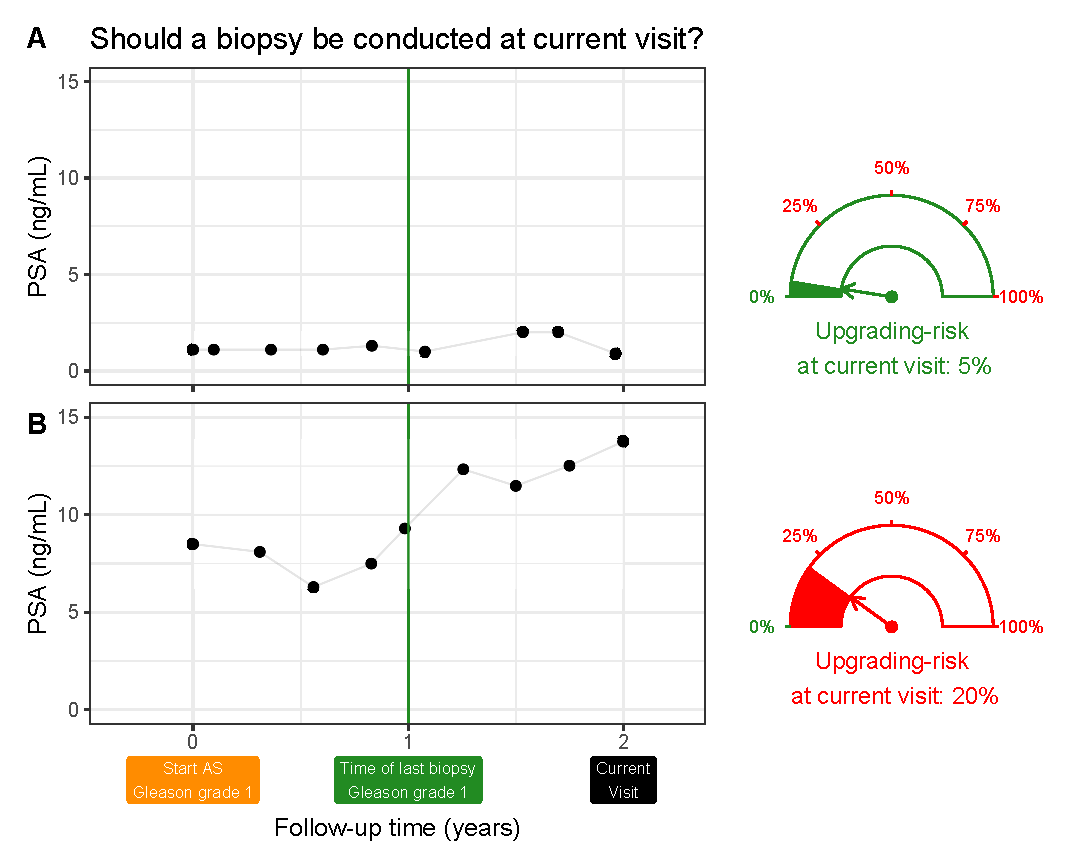
\includegraphics[width=\columnwidth]{images/riskBasedExample.eps}}
\caption{\textbf{Motivation for upgrading-risk based personalized biopsy decisions}: To utilize patients' complete longitudinal data and results from previous biopsies in making biopsy decisions. For this purpose, we first process data using a statistical model and then utilize the patient-specific predictions for risk of Gleason upgrading to schedule biopsies. For example, Patient~A (\textbf{Panel~A}) and B (\textbf{Panel~B}) had their latest biopsy at year one of follow-up (green vertical line). Patient~A's prostate-specific antigen (PSA) profile remained stable until his current visit at year two, whereas patient~B's profile has shown a rise. Consequently, patient~B's upgrading-risk at the current visit (year two) is higher than that of patient~A. This makes patient~B a more suitable candidate for biopsy than Patient~A. Risk estimates in this figure are only illustrative.}
\label{fig:riskBasedExample}
\end{figure}

This work is motivated by the problem of scheduling biopsies in AS. We have two goals. First, we want to assist practitioners in using clinical data in biopsy decisions in a statistically sound manner. To this end, we plan to develop a robust, generalizable statistical model that provides reliable individual upgrading-risk in AS. Subsequently, we will employ these predictions to derive risk-based personalized biopsy schedules. Our second goal is to enable shared decision making of biopsy schedules. We intend to achieve this by allowing patients and doctors to compare the \emph{burden} and \emph{benefit} (Figure~\ref{fig:delay_explanation}) of opting for personalized schedules versus periodical schedules versus schedules based on clinical data. Specifically, we propose timing and number of planned biopsies (more/frequent are burdensome), and the expected time delay in detecting upgrading (shorter is beneficial) for any given schedule. While fulfilling our goals, we want to capture the maximum possible information from the available data. Hence, we will use all repeated measurements of patients, previous biopsy results, baseline characteristics, and keep our model flexible to accommodate novel biomarkers in the future. To fit this model, we will utilize data of the world's largest AS study, Prostate Cancer Research International Active Surveillance (PRIAS). To evaluate our model, we will externally validate it in the largest six AS cohorts from the Movember Foundation's Global Action Plan (GAP3) database~\citep{gap3_2018}. Last, we aim to implement the validated model and methodology in a web-application.